\chapter{Go Endgames Using Ad-Hoc Mathematics}
\epigraph{
  Combinatorial game theory captures an~essential part of~what Go is about.
  I think that in one form or another, it will become a~key component of~all successful future Go programs.%
  \footnotemark
}{Martin~\cite{Muller1995computer}}
The ancient game of~Go offers astounding complexity:
the board size, the quantity of~possible moves and the average game length produce an~astronomical number of~valid positions.
More than in~any other classic game, human intuition plays a~vital role for a~successful play:
Go offers abundance and richness of~geometrical, combinatorial and logical structure, ready to be exploited by human players.
\footnotetext{
  In fact, this prognosis is misaligned:
  AlphaGo, the most successful Go program designed so far, uses no Go-specific knowledge.
  To compare \Mueller's prediction with current trends, consult the Note on page~\pageref{note:CGTvsAlphaGo} or Chapter~\ref{ch:AlphaGo}.
}

\note{
  This chapter is based on the work of Martin~\Mueller{} (\cite{Muller1995computer}) submitted as a~doctoral thesis at ETH \Zurich.
  Since the focus of~our survey are imperfect-information games rather than Go, the chapter heavily derives from the mentioned work.
}

Martin~\Mueller{} in~(\cite{Muller1995computer}) reports that (at that time) Go programs ``comprehend only the most basic concepts of~Go'' and that
``to make progress, [he~feels] it is necessary both to encode more Go-specific knowledge and to push forward the application of~theories such as combinatorial game theory to Go''.
Here follows the summary and the results of~his endeavors.

\section{Why Focus on Go Endgames?}

In his dissertation, Martin~\Mueller{} mentions the following advantages of~Go endgames for research:
\begin{itemize}
  \item The situation towards the end of~game becomes clearer.
    This simplification helps to study Go in~an easier and more controlled way.
  \item Some endgame positions allows for an~exact solution within reasonable time.
  \item Understanding parts of~board improves the understanding of~the whole game.
    Such partial evaluations aids various heuristics for solving the full board.
    Humans reason similarly: by~observing the score since the early midgame, they decide based on~such a~heuristic analysis (\cite{Takagawa85}).
  \item Methods and techniques for partitioning, searching and scoring during endgame are frequently also applicable to the midgame and opening.
  \item Endgames provide a~simplified, more manageable sub-domain allowing the use of~stronger theoretical models than the larger, more general problem.
\end{itemize}

\section{Partitioning into (Sub)games and Playing The Game-Sum}
{
  \setlength{\epigraphwidth}{0.4\textwidth}
  \epigraph{
    Divide et impera.
  }{Philip II of~Macedon}
}%
A~typical Go position contains several \emph{subgames} (local scenes) suitable for independent analysis.
Initially, the subgames have no influences on~one another due to their mutual distance.
As the game progresses, nevertheless, they gain the crucial role due to a~clearer board partition with walls of~safe stones:
\begin{figure}[H]
  \centering
  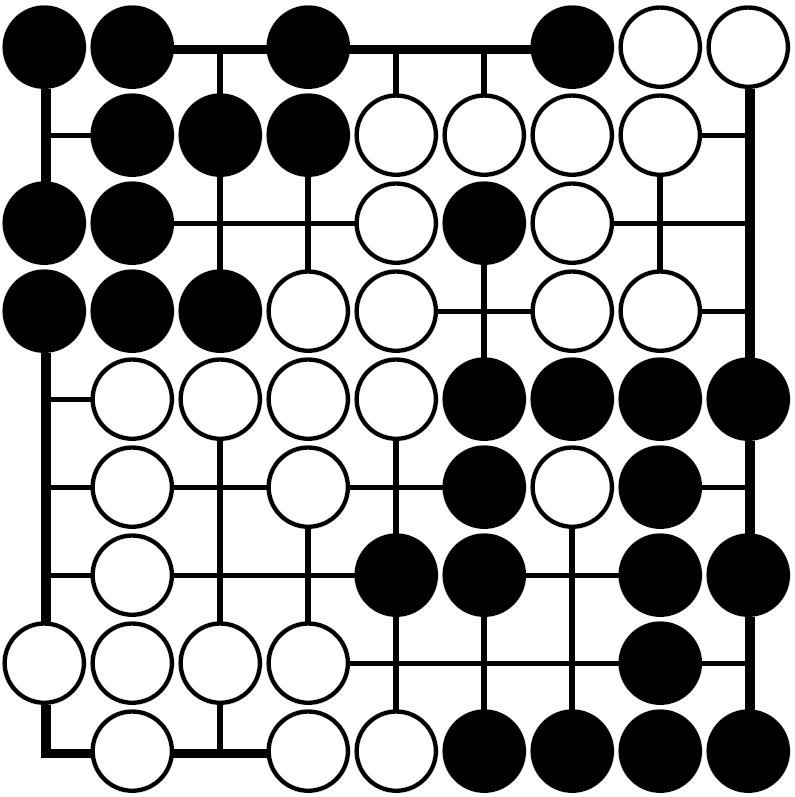
\includegraphics[width=.4\textwidth]{../img/late_endgame_Go_position_suited_for_exact_analysis.png}
  \captionWithCite{An~immortal wall enabling an exact analysis during late endgame}{Muller1995computer}
  \label{fig:immortal-wall}
\end{figure}
No move can have any influence across these ``immortal'' walls and significant parts of~the board definitely belong to one of the players.
The connected components of~remaining stones define local subgames independent from each other.

In the opening and midgame, only approximate partitioning can be available.
In the endgame, conversely, the partition gets more precise:
the status of~all big groups has been settled, and the outlines of~territories are clear.
If each local game is simple enough to~analyze completely (such as in Figure~\ref{fig:immortal-wall}), combinatorial game theory can compute an~optimal move for the full board position.
(\cite{Muller1995computer})

This is the general procedure of~(\cite{Muller1995computer}) for playing Go as a~sum of~local games:
\begin{enumerate}
  \item Board partition: find safe blocks, safe territories, and local areas.
  \item Generate local game trees in each area.
  \item Evaluate local terminal positions.
  \item Transform local game trees into mathematical games (and simplify games).
  \item Find an optimal move in the (combinatorial game theory) sum-game and play it.
\end{enumerate}
\Mueller{} proposes heuristic algorithms for playing the entire game, and exact algorithms for late endgame positions.

Undoubtedly, the task of~solving endgames in 1995 (at the age of Computer Go's infancy) already played a~vital role.

\section{Combinatorial Game Theory for the Game of~Go}

\epigraph{
  [$\dots$]
  You get surreal numbers by~playing games.

  I used to feel guilty in Cambridge that I spent all day playing games, while I was supposed to be doing mathematics.
  Then, when I discovered surreal numbers, I realized that playing games IS math.
}{John Horton Conway}
\Mueller{} suggests to replace the ``standard model'' of~computer Go by a~sum-game model.

Here follows some of~the general benefits and problems of~the sum-game model for computer Go as listed in~(\cite{Muller1995computer}):

\medskip

\underline{Benefits}
\begin{itemize}[+]
  \item suitability to the knowledge and style of~Go programs at that time:
    local fighting, surrounding territories$\dots$
  \item the reuse of~local game analysis for higher quality game-play
  \item simplification of~move generation and position evaluation
  \item translation of~Go terms into the theory, without any need for~separate programming
  \item evaluation of~the opponent's endgame moves
  \item assessment of~sufficiently good moves even with a~\emph{reduced} local game database
  \item position's game-theoretic value computed long before the end
  \item opportunities for parallelism:
    independent local searches, evaluation and operations on mathematical games$\dots$
  \item perfect computer play in~late endgame
\end{itemize}

\underline{Obstacles}
\begin{itemize}[-]
  \item required accurate board partition and recognition of~dependencies
  \item the common issues of~selective search:
    misleading evaluation due to missing crucial moves in~complicated games
  \item the lack of~long-range full-board planning:
    ``This is probably not a~big issue until programs reach amateur Dan or even professional level.''%
    \footnote{For an~update on the situation today, see Chapter~\ref{ch:AlphaGo}.}
\end{itemize}

The strict endgame analysis of~(\cite{Muller1995computer}) is additionally impossible, when one of~the following \underline{limitations} is met:
\begin{itemize}[-]
  \item \textbf{partition:}
    There is insufficient amount of~blocks that can be proven safe.
    Some of~the areas are hence too large for~the complete search.
  \item \textbf{summation:}
    No~move with dominating incentive exists, and both summing and partial search would take too long.
  \item \textbf{Ko:}
    Combinatorial game theory relies on the independence of~local subgames.
    In the case of~Ko, the independence is broken:
    a~locally bad move may be globally best if it serves as a~Ko threat (recall Section~\ref{sec:Go}).
    \Mueller{} mentions in~1995 there was ongoing research to generalize the theory for handling Kos.
  \item \textbf{Unneccessary complexity in ``straightforward'' situations:}
    In cases where the focus of~play is straightforward (i.e. only one local situation is relevant), combinatorial game theory introduces additional complexity.
    Namely, CGT investigates moves for~both players in~this and every other position.
\end{itemize}

\section{Board Partition and Subgame Dependencies}
\epigraph{
  Independence?
  That's middle class blasphemy.
  We are all dependent on~one another, every soul of~us on Earth. 
}{George Bernard Shaw}
In addition, (\cite{Muller1995computer}) mentions several further obstacles of~the sum-game model, caused by~the heuristic board partition:

\begin{itemize}[-]
  \item the impossibility of a~perfect, precise split:
    During the opening or~midgame, there are almost no surrounded spaces, and moreover, the surrounding stones would not be invulnerable yet.
    Heuristics is needed for board partition to split the imperfectly surrounded areas.

  \item the infeasibility of~exhaustive search in still large subgames:
    The program is obliged to give a~move in a~few seconds or minutes.
    However, there still remain areas intractable for an~exhaustive search.

    In such subgames, \Mueller{} employs \emph{selective search} method.
    He limits the number of~generated moves and stops the search before reaching a~terminal position.
    For each local game, nodes to expand need to be decided and \emph{expert modules for search and evaluation} need to be selected.
    A~post-processing stage handles detected dependencies between games.

  \item the dependencies between the resulting subgames, which arise with the previously mentioned heuristics:
    The effect of~such dependencies differs widely:
    often it is so small that independence is a~useful approximation.
    In cases when a~move works as a~\emph{double threat} however, dependency analysis is crucial.

    Trivial strategies to overcome dependencies involve:
    \begin{itemize}
      \item ignoring the dependency, as if the games were independent,
      \item proving that the dependency does not affect the value of~the sum, or play of~the sum game,
      \item merging mutually dependent local games, then re-search the combined game, possibly using previously generated information on single games,
      \item analyzing the interaction between local games, then use a~specialized theory to compute the joint game value.
    \end{itemize}
\end{itemize}

Hence, the sum game model makes the best sense during the endgame part.
This general principle is as well applicable in poker:
we wait until the late stage of~the game, when it has greater impact to refine and re-solve the reached endgames.

\section{Local Search and Evaluation in the Endgame}
\epigraph{
  True genius resides in~the capacity for~evaluation of~uncertain, hazardous, and conflicting information. 
}{Winston Churchill}
Once the board is partitioned, the algorithm of~(\cite{Muller1995computer}) for converting a~Go endgame into a~combinatorial game follows these steps:
\begin{enumerate}
  \item Generate local game trees:
    all legal moves are generated from point of~both players, with exceptions~of:
    \begin{enumerate}[(a)]
      \item \emph{pruning rules}%
        \footnote{Compare with \emph{policy networks} of~AlphaGo in Chapter~\ref{ch:AlphaGo}.},
        e.g. pruning dominated subgame trees:
        the evaluation of~nodes allows for pruning moves dominated by other moves.
        Moves with a~dominating alternative are labelled as~\emph{locally bad moves}.

      \item \emph{termination rules} for static evaluation of a~position, without further tree expansion%
        \footnote{Compare with \emph{value network} of~AlphaGo in Chapter~\ref{ch:AlphaGo}.}
    \end{enumerate}

  \item Score local terminal positions:
    \begin{enumerate}[(a)]
      \item \emph{scoring}%
        \footnote{See Section~\ref{sec:Go}.}
        comes in two widely-accepted flavors, namely
        \begin{enumerate}[$\diamondsuit$]
          \item Chinese variant, which counts stones and empty points belonging to either color,
          \item Japanese variant, which counts territory and prisoners.
        \end{enumerate}
        Both variants have straightforward implementation because safe stones, dead stones, territories and neutral points are known exactly in~the endgame.

      \item \emph{terminal positions} can be recognized by
        \begin{enumerate}[$\diamondsuit$]
          \item no more legal moves,
          \item no more good moves,
          \item the value of~position already known from the transposition table, pattern, or local position database.
        \end{enumerate}
        A~position is additionally considered terminal, once we can ascertain its value from another source.
        Such a~value can be any value in~the sense of~mathematical games.

        Non-terminal positions may have a~constant value as well, if the outcome is the same no matter who plays first, but this has to be proven using search.
    \end{enumerate}

  \item Evaluate local games as mathematical games.
    Explicitly, evaluate terminal positions, and back up the values in~the tree, resulting in a~mathematical-game evaluation of~each node.

    Even though the program reaches a~solved position, (\cite{Muller1995computer}) notes that a~``suicidal'' opponent may later cause great troubles, by endangering his immortal stones.
    Such an~act would violate the assumptions on~board partitioning and give rise to~new unexpected positions with rather complicated optimal play.

  \item Select an~option in the resulting (abstract) sum-game.
  \item Translate the chosen option in~the abstract game into a~corresponding move in~Go.
    This move is taken as~the first move with sufficient \emph{incentive} (recall Section~\ref{sec:CGT}).
\end{enumerate}

\begin{figure}[H]
  \centering
  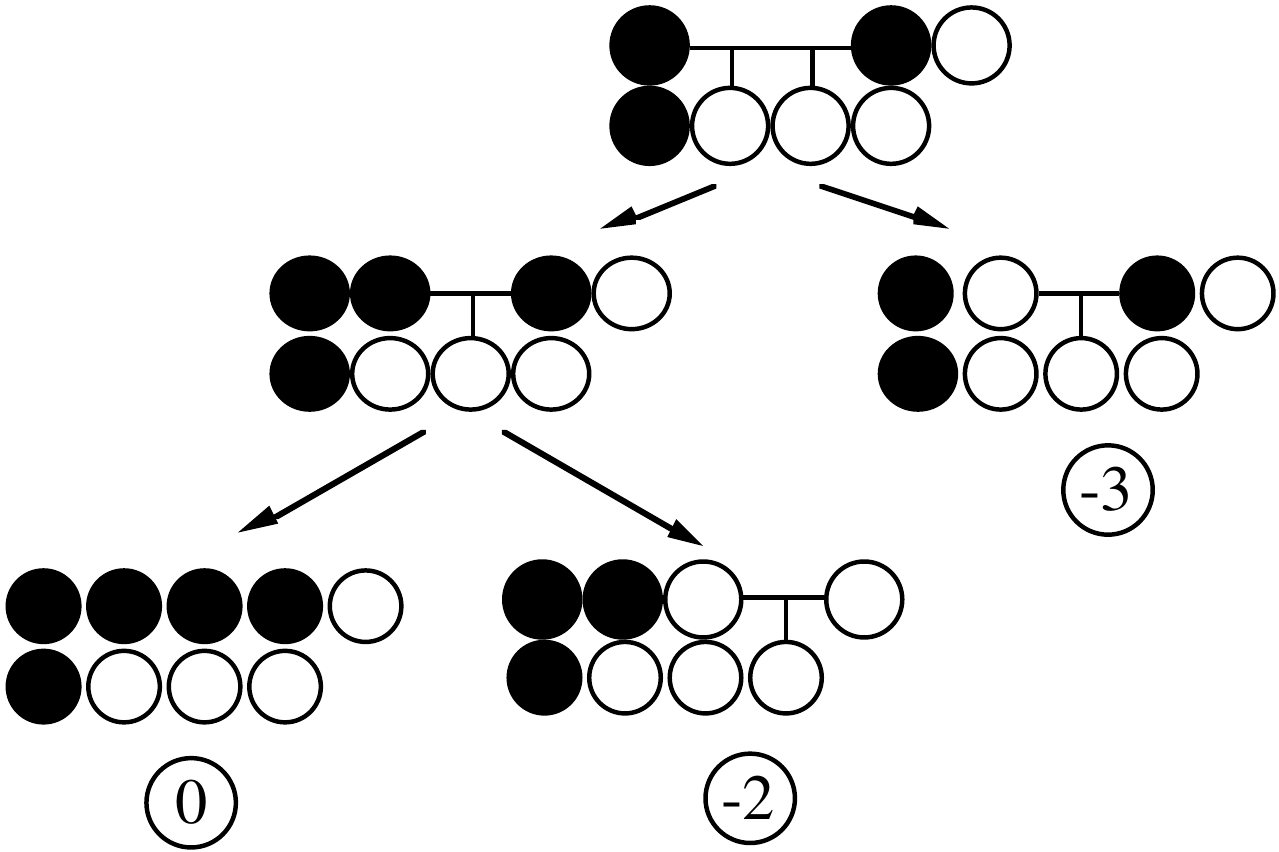
\includegraphics[width=.5\textwidth]{../img/Go_search_tree.png}
  \captionWithCite{Local game tree with evaluation of terminal nodes}{Muller1995computer}
\end{figure}

\section{Storing Search Results into Database}
\epigraph{
  I'm blessed with very fast memorization skills, so I don't have to read it too far in advance.
}{Jaimie Alexander}
Search and analysis produce the complete description of possible endgame plays, facilitating the perfect strategy.
The results are stored in a~\emph{database of~local positions}.
Local subgames during a~live play are then matched one-to-one to a~set of~database positions.
The value of a~full board position is the sum of~local position values and an~algorithm for sum-game evaluation selects the best available response.

A~version with lower memory requirements is implemented as well.
This is achieved by~saving only a~selection of~positions, and in~case the subgame is missing in the database, re-doing the search.

An~important question is what to store.
Table~\ref{tab:db-loc-games} lists some possible answers:
\begin{table}[!htbp]
  \centering
  \begin{tabular}{ |p{.45\textwidth}|p{.48\textwidth}| } 
    \hline
    \textbf{Type of database} & \textbf{Content} \\
    \hline
    Full                            & $\dots$every position discovered during exhaustive search \\
    Color-complete (Black or White) & $\dots$every position reachable by~non-dominated moves of~the color and arbitrary opponent's moves (pruned bad moves of~the color) \\
    Optimal                         & $\dots$at~least one position corresponding to~every non-dominated option of~every reachable position (guaranteed optimal play from every position in~database) \\
    Sufficiently good               & $\dots$guaranteed optimal score from a~starting position (might fail to exploit some opponent mistakes) \\
    \hline
  \end{tabular}
  \captionWithCite{Possible database variants of~local games}{Muller1995computer}
  \label{tab:db-loc-games}
\end{table}

One needs to make a~trade-off between re-computation time and storage space.
A~sensible solution is to~store only complicated moves in~the database, and re-calculate the rest when necessary.
It is a~good idea to save only the information whether a~move is locally good or bad, but discard \emph{refutations}\footnotemark.
\footnotetext{the trees proving that bad moves are inferior}
Such a~type of~database is robust against a~good opponent;
however, it suffers from a~play of a~locally bad opponent.
This~rare situation would call for the re-computation of~a~subtree in order to find a~refutation.

The number of~possible moves in an $n$-point area is approximately $2n$ ($n$ for each player), and such a~play generates a $n-1$ point area.
Whence, the size of~the game tree is approximately $2n\cdot2(n-1)\cdot \ldots \cdot2 = 2^n n!$ nodes.
Such a~combinatorial explosion makes even fairly small endgames prohibitively expensive.
\Mueller{} overcomes this hardness with a~transposition table.
A~\emph{transposition table} detects identical board positions, reducing the size of~the search space from $\approx 2^n n!$ to $3^n$ states (see the comparison in Table~\ref{tab:reduction-transp-tab})
\begin{table}[!htbp]
  \centering
  \begin{tabular}{ |rrr| }
    \hline
    \textbf{$n$} & \textbf{$2^nn!$} & \textbf{$3^n$} \\
    \hline
    1	&	2	&	3 \\ 
    2	&	8	&	9 \\ 
    3	&	48	&	27 \\ 
    4	&	384	&	81 \\ 
    5	&	3840	&	243 \\ 
    6	&	46080	&	729 \\ 
    7	&	645120	&	2187 \\ 
    8	&	10321920	&	6561 \\ 
    9	&	185794560	&	19683 \\ 
    10	&	3715891200	&	59049 \\ 
    \hline
  \end{tabular}
  \caption{Reduction of search space by transposition table}
  \label{tab:reduction-transp-tab}
\end{table}

\section{Pattern Learning}
{
  \setlength{\epigraphwidth}{0.55\textwidth}
  \epigraph{To understand is to~perceive patterns.}
  {Isaiah Berlin}
  \epigraph{When patterns are broken, new worlds emerge.}
  {Tuli Kupferberg}
}%
Pattern recognition is one of~the key components of~AlphaGo (see Chapter~\ref{ch:AlphaGo}).
Arguably, the program's success might be partially attributed to learning Go patterns from human expert plays.

For comparison, (\cite{Muller1995computer}) hails computer Go as \emph{a~vehicle for research in~visual perception, machine learning and neural networks} (based on~\cite{Wilcox79}; \cite{Enderton1991golem}; \cite{Stoutamire1991machine}; \cite{Schraudolph1994temporal}).

Being introduced just and only to~Go rules, learning programs can typically pick up basic Go principles, such as saving a~stone from capture, and familiarize themselves with~low-level game concepts.
However, these concepts and principles have already been integrated into~other far superior \emph{expert-based programs}.
Neural networks are therefore more adapt at~playing locally good shapes, but possess no~idea when to play it.%
\footnote{This assertion especially has changed thanks to~AlphaGo.}
These systems are vulnerable to other Go agents with better knowledge of~tactics.

In the end, (\cite{Muller1995computer}) suggests \emph{pattern matching} as a~promising means for the significant advancement of~computer Go.

\section{Contributions of~Combinatorial Game Theory to Go Endgames}

The doctoral thesis (\cite{Muller1995computer}) highlights following contributions to general computer science:
\begin{itemize}
  \item ``Scientists are fascinated by problems which can be stated simply, yet are hard to solve.
    Computer Go is a~prime example.
    We have brought the divide-and-conquer approach, a~fundamental paradigm of~computer science, to bear on computer Go.''

  \item ``The application of a~sophisticated mathematical theory to computer Go provides an~example of~algorithms for a~nontrivial decomposition of a~complex problem.''
\end{itemize}
and contributions to computer Go:
\begin{itemize}
  \item ``We have implemented a~\emph{late endgame player}, a~niche where program play surpasses human play in both speed and exactness.
    We did this by applying concepts from combinatorial game theory to Go.
    The program plays a~wide variety of`late endgame positions perfectly.''

  \item ``We have developed algorithms for board partition and dependency analysis.
    The central idea of~board partition has been used both in a~program following a~traditional model, and in a~program based on the sum game approach.''
\end{itemize}
Hence, the work employs a~technique of~applying an~elaborate mathematical theory (of~combinatorial game theory) to deal with the endgame phase.
In particular, CGT is used to ``connect'' individual relevant subgames, which may be solved independently.

As we will see later, the situation in the case of~Poker is slightly more delicate:
the imperfect-information property prevents us from using an~immediate divide-and-conquer approach.
Instead, we will \emph{augment} the information by saturating it with additional game states (see Chapter~\todo).

\note{
  \label{note:CGTvsAlphaGo}
  It is also interesting to compare the method of~(\cite{Muller1995computer}) with the modern approach of~\emph{AlphaGo}:
  the ad-hoc Go-specific knowledge is replaced with general-learning neural networks and the probabilistic \emph{Monte Carlo Tree Search} algorithm.
  Such a~combination has the capability to surpass professional human players at the highest ranks.
  On top of that, this solution can be adapted to other games without substantial modifications.
  As long as there is an~abundance of~available data, the system can always be trained with no need to imbue it with any game-specific knowledge.
  See Chapter~\ref{ch:AlphaGo} for more details.
}
